\chapter[Benchmarking, Environment Setup and Characterization of the PMU]{Benchmarking, Environment setup and characterization of the Sandy Bridge Performance Measurement Unit}\label{chapter:envsetup}

This chapters introduces the environment used in the execution of the developed solution and the benchmarks that will be used as observed programs to test the functioning of such solution. The second part of this chapter presents the first experimental results explain how the setting of the sampling configuration influences the obtained samples.

\section{Testing Environment}\label{section:runningenv}
The testing unit consists of a host with two NUMA nodes joined by a QPI link. Every node is an Intel Xeon E5 compliant to the Intel Sandy Bridge-EP microarchitecture. Every node contains 8 physical cores, where every core has a clock speed of 2.6 GHz. However, because of the Hyper threading available in this processor, the operating system sees 16 cores for every NUMA node, making it 32 cores in total. The host altogether has a RAM capacity of 128 GB. All the tests were performed under the 3.16 version of the Kernel.

\section{Employed Benchmarks}\label{section:emplybmchs}

\subsection{Distgen}\label{section:distgen}
The first algorithm to test aims to explore the behavior of the page movement functionality in a simple application which accesses a memory location. The simplest scenario would be to implement a loop that traverses a consecutive memory space sequentially and use the SPM tool to evaluate the performance of the developed algorithm. The objection to this idea is that because of the hardware prefetcher present in most of the modern processors, this application will execute very quickly. The first modification would be to access a random memory location in the memory space for each iteration, instead of the sequential access proposed first. The random location can be chosen by making use of the \textbf{random} call, present in the stock C library. The traversal executes slower than the sequential access as predicted, but the problem that was found is that the C random function has locks in its implementation that become a considerable bottleneck.

Because of the implementation with locks of the C function, what is needed is a random number generator faster than the stock random function. It does not matter if the random generation is less strict, because this generation is only needed to avoid engaging the hardware prefetcher and for this purpose \textbf{Distgen} comes into play. Distgen, coded by Josef Weidendorfer, whose availability is presented in code listing \textit{original distgen}, is an algorithm that transverses a memory area in a sequential or pseudo random manner where the latter mode is executed with low overhead. The execution command for distgen is as follows:
\begin{center}
\texttt{distgen [-p] [n-iterations] [size]}
\end{center}

Where the presence of the -p indicates that the traversal will use the pseudo random sequence, when not present it will transverse the space in a streaming fashion. The optional parameter n-iterations determines how many times the space will be traversed and the size parameters determines the size of the domain to iterate through. If any of these parameters is not specified the defaults will be applied.

\subsection{LAMA-CG}\label{section:Lama}
LAMA (www.liblama.org) is an open source library written in C++ and developed by the SCAI Institute of the Fraunhofer Society. Its objective is to ease the use of applications that require sparse and dense linear algebra functionality. It supports many parallel computing models such as MPI and NVIDIA GPUs, but its use on this document is limited to the single node case using OpenMP. The application to be tested is a conjugate gradient solver (CG) which makes use of the LAMA functionality. The reason it was chosen is because it is an algorithm frequently found in high performance computing applications, with a more realistic functionality than distgen.
The invocation of the cg functionality is done with the following command:\\
\begin{center}
\texttt{cg\_solver.exe LOG TX}
\end{center}

Where LOG is a logging option not used in this project and the X after the T represents the number of threads to run the project with.

\section{Characterization of an Intel Sandy Bridge Performance Measurement Unit}\label{section:pmu-charzn}
This section presents some measurements that allow to give a better understanding of how the configuration parameters of the CPU guide its behavior. All the measurements were taken with distgen as the observed process.


\subsection{Latency Weight Distribution}\label{subsection:pmu-latwei}

\begin{figure}[th]
	\centering
		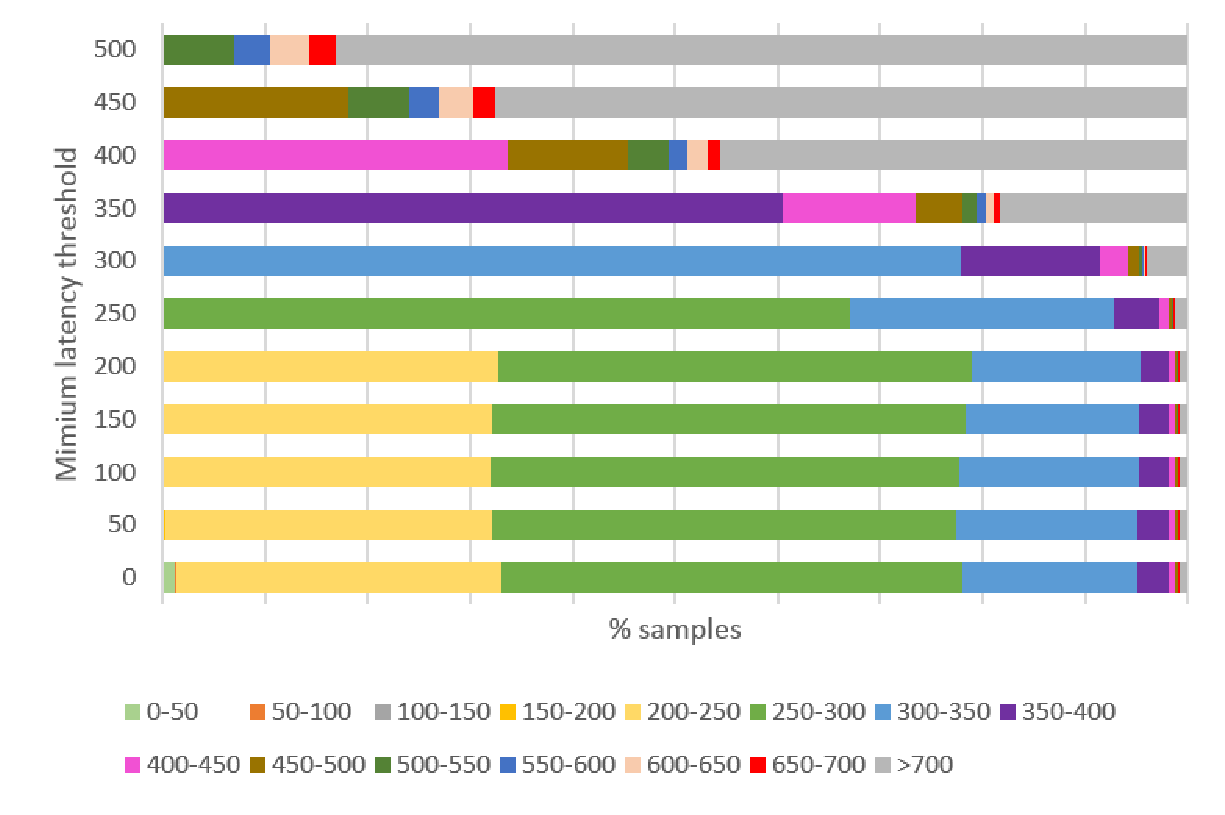
\includegraphics[width=.8\textwidth]{figures/latencydistw20.eps}
		\caption[Sample weight distribution with a period of 20 instructions per sample.]{Sample weight distribution with a period of 20 instructions per sample for different minimum weight thresholds using distgen as the observed process. }
		\label{fig:latencydistw20}
\end{figure}

\begin{figure}[h]
	\centering
		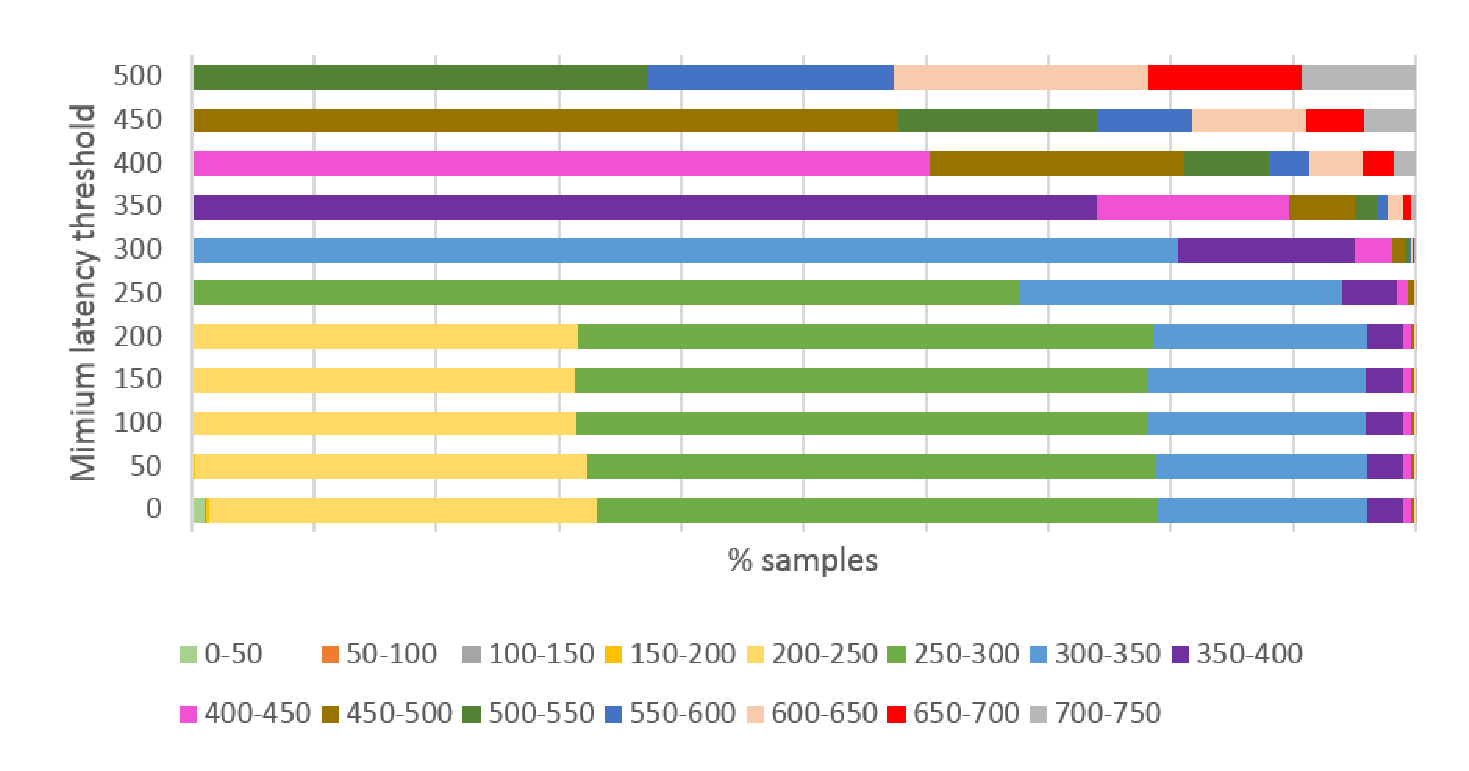
\includegraphics[width=.8\textwidth]{figures/latencydistw200.eps}
		\caption[Sample weight distribution with a period of 200 instructions per sample.]{Sample weight distribution with a period of 20 instructions per sample for different minimum weight thresholds using distgen as the observed process.}
		\label{fig:latencydistw200}
\end{figure}


The sample latency distribution shows the distribution of the latency values when the sample is taken under a certain period and minimum weight threshold. Every bar corresponds to a specific latency weight threshold and all the bars on the same picture correspond to the same sampling period. The weight of every sample is placed in its corresponding interval and every color corresponds to the percentages of samples belonging to that interval in proportion to the overall number of samples taken.  The results are shown in figures \ref{fig:latencydistw20} and \ref{fig:latencydistw200}, which correspond to the periods of 20 and 200 instructions per sample. The other figures are omitted because of an almost identical distribution in relation to the ones shown

There are some insights that these graphics deliver: First, the working of the minimum weight threshold works, for instance all the distributions with a weight under 250, it can be seen how the samples with weights between 200 and 150, 250 and 300 and 300 and 350 dominate the distribution but with filtering values above that value the samples in those intervals no longer appear. Second, The distribution of the samples is very similar throughout all the sampling periods, which shows that it is independent of the sampling period values. Third, In this algorithm memory latency is an important cause for slow performance, taking into account that local memory requests are served with latencies of tens of clock cycles, at most.


\subsection{Number of Obtained Samples}\label{subsection:pmu-obtainedsamp}


\begin{figure}[th]
	\centering
		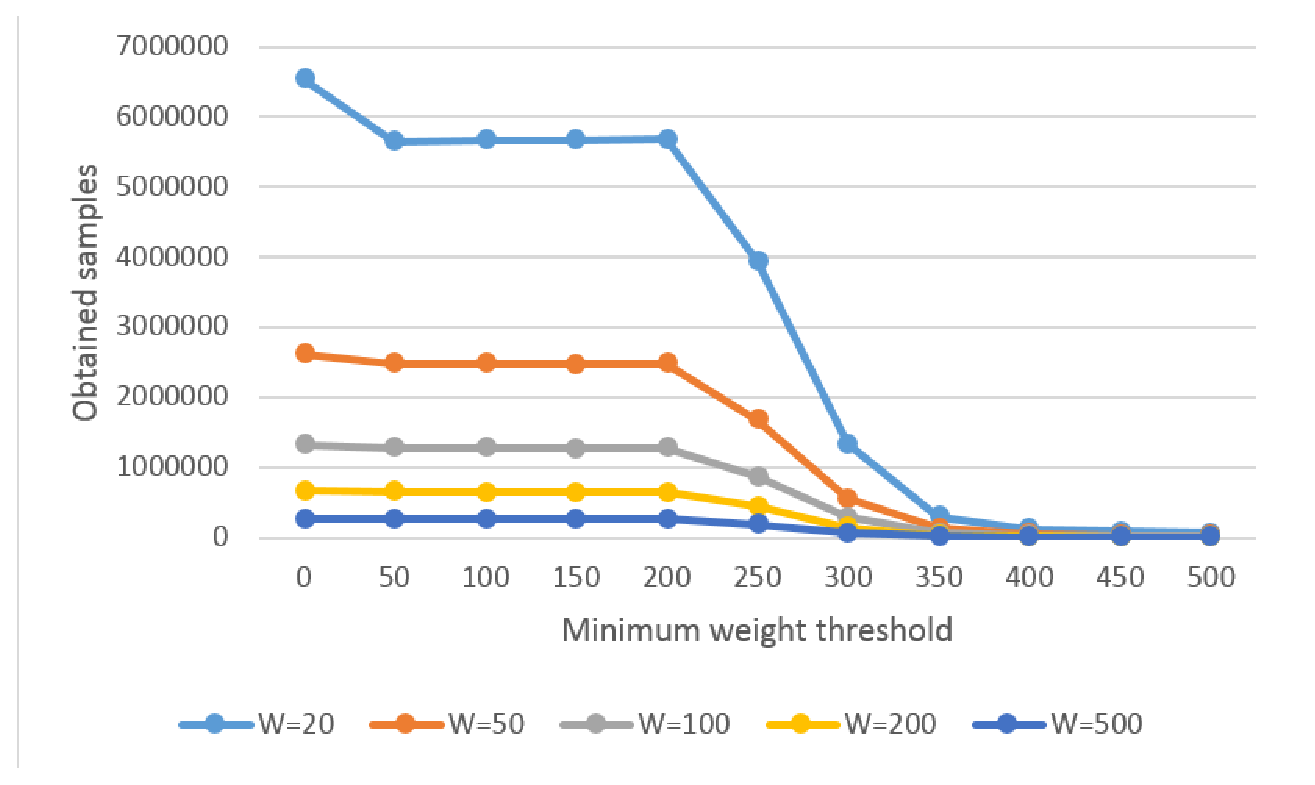
\includegraphics[width=.8\textwidth]{figures/number-samples.eps}
		\caption{Number of samples obtained for different period and weight threshold settings with distgen-random as the observed process.}
		\label{fig:pmu-obtainedsamp}
\end{figure}

The sample distributions omit a very important type of information, which is the number of samples acquired for every period and weight threshold combination. Knowing how many samples were obtained is important because a high number of samples helps the SPM tool form a good idea of the memory access behavior of the observed process, but on the other hand every sample received must be processed, which in turn implies higher CPU consumption that could be taken away from the supervised process. 

Figure \ref{fig:pmu-obtainedsamp} shows how the number of samples taken reacts to changes in the sampling period and minimum weight threshold. Because a higher weight threshold implies discarding a bigger number of samples under a certain value, this relationship decreases. This experiment also confirms that a low period is directly related to an increasing number of samples.

\subsection{Frequency of Page Accesses}\label{subsection:pmu-freqpgacc}

\begin{figure}[th]
	\centering
		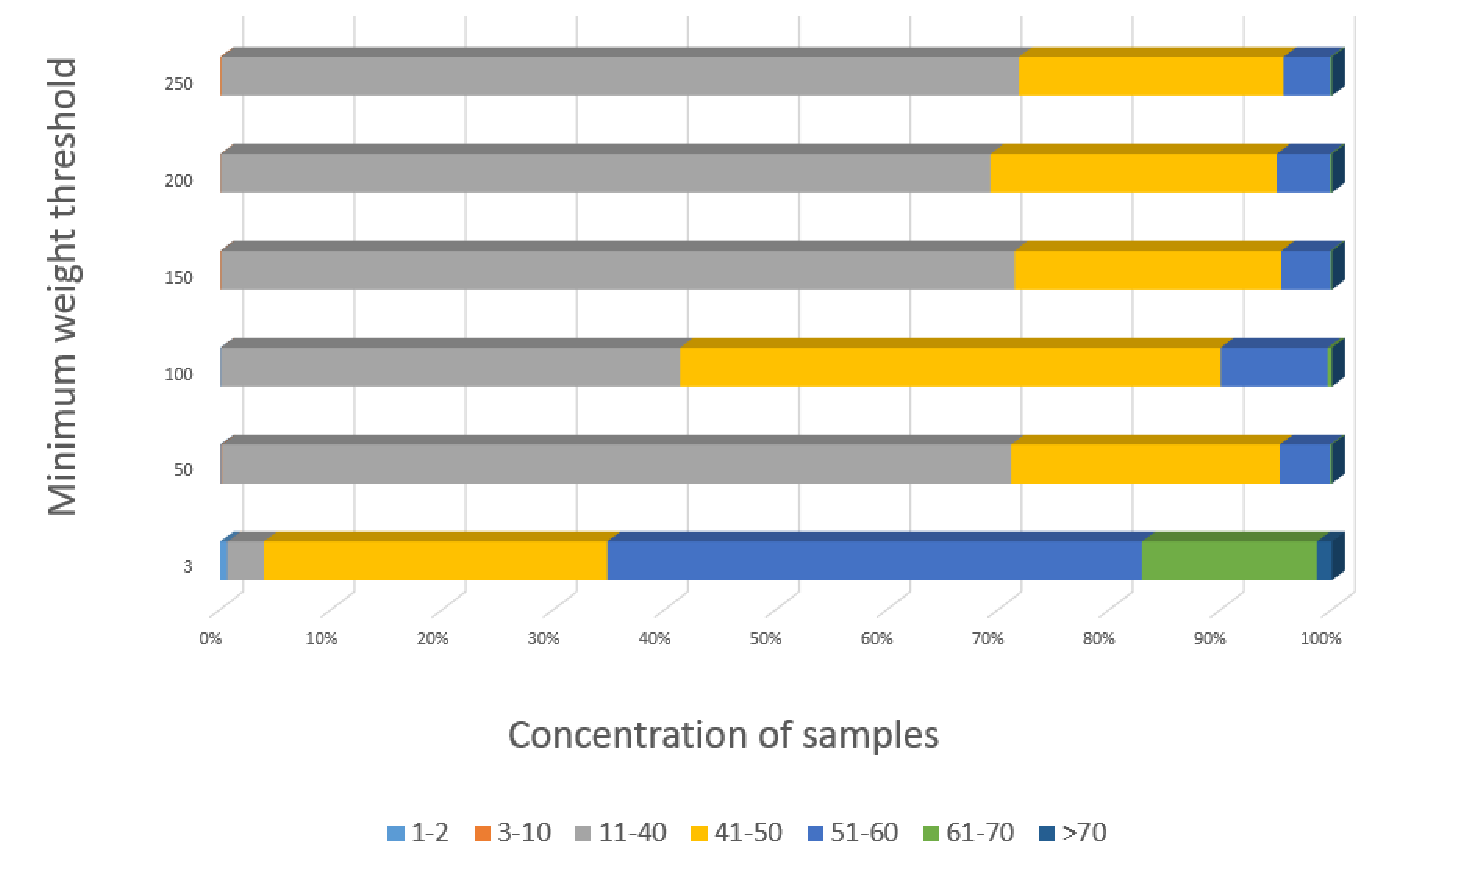
\includegraphics[width=.8\textwidth]{figures/pagetouch-dgenrdm.eps}
		\caption{Frequency of page accesses: Percentage of pages that were accessed a given number of times during a run of the distgen-random algorithm.}
		\label{fig:pmu-concentsamp-dgenrdm}
\end{figure}

\begin{figure}[th]
	\centering
		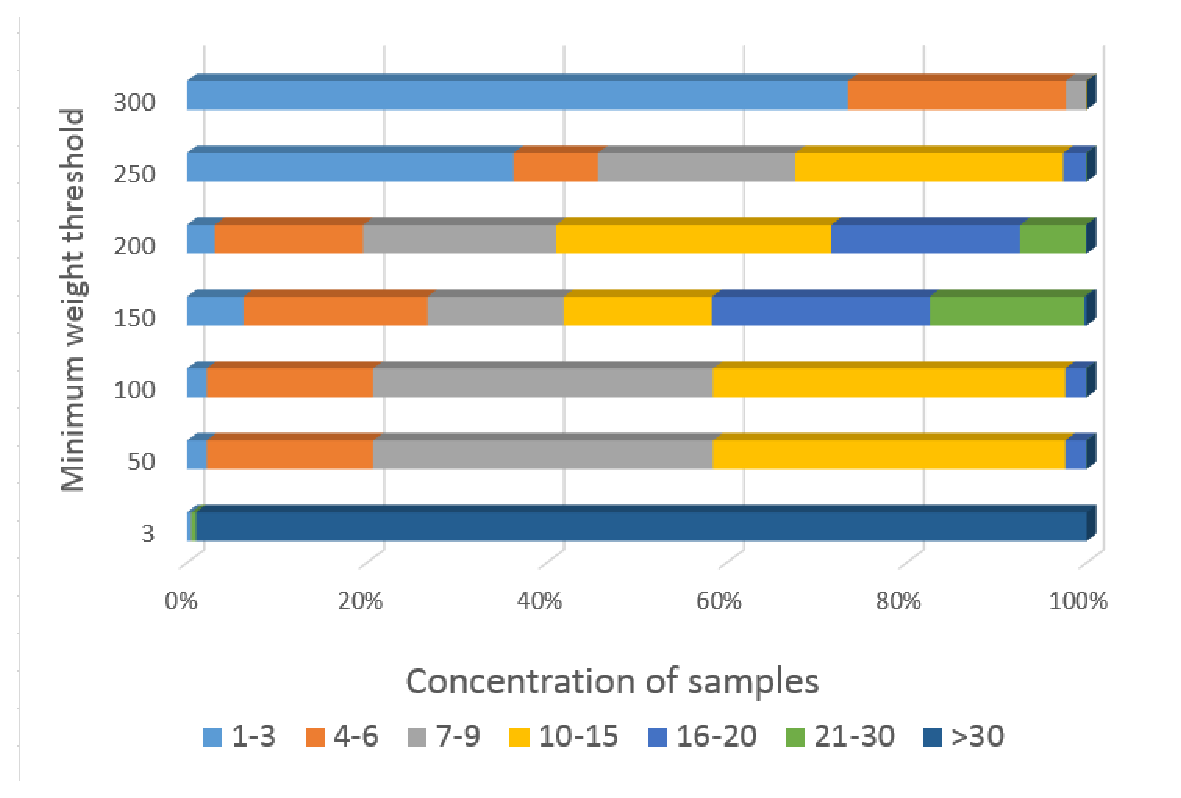
\includegraphics[width=.8\textwidth]{figures/pagetouch-dgenser.eps}
		\caption{Frequency of page accesses: Percentage of pages that were accessed a given number of times during a run of the distgen-sequential algorithm.}
		\label{fig:pmu-concentsamp-dgenser}
\end{figure}

\begin{figure}[th]
	\centering
		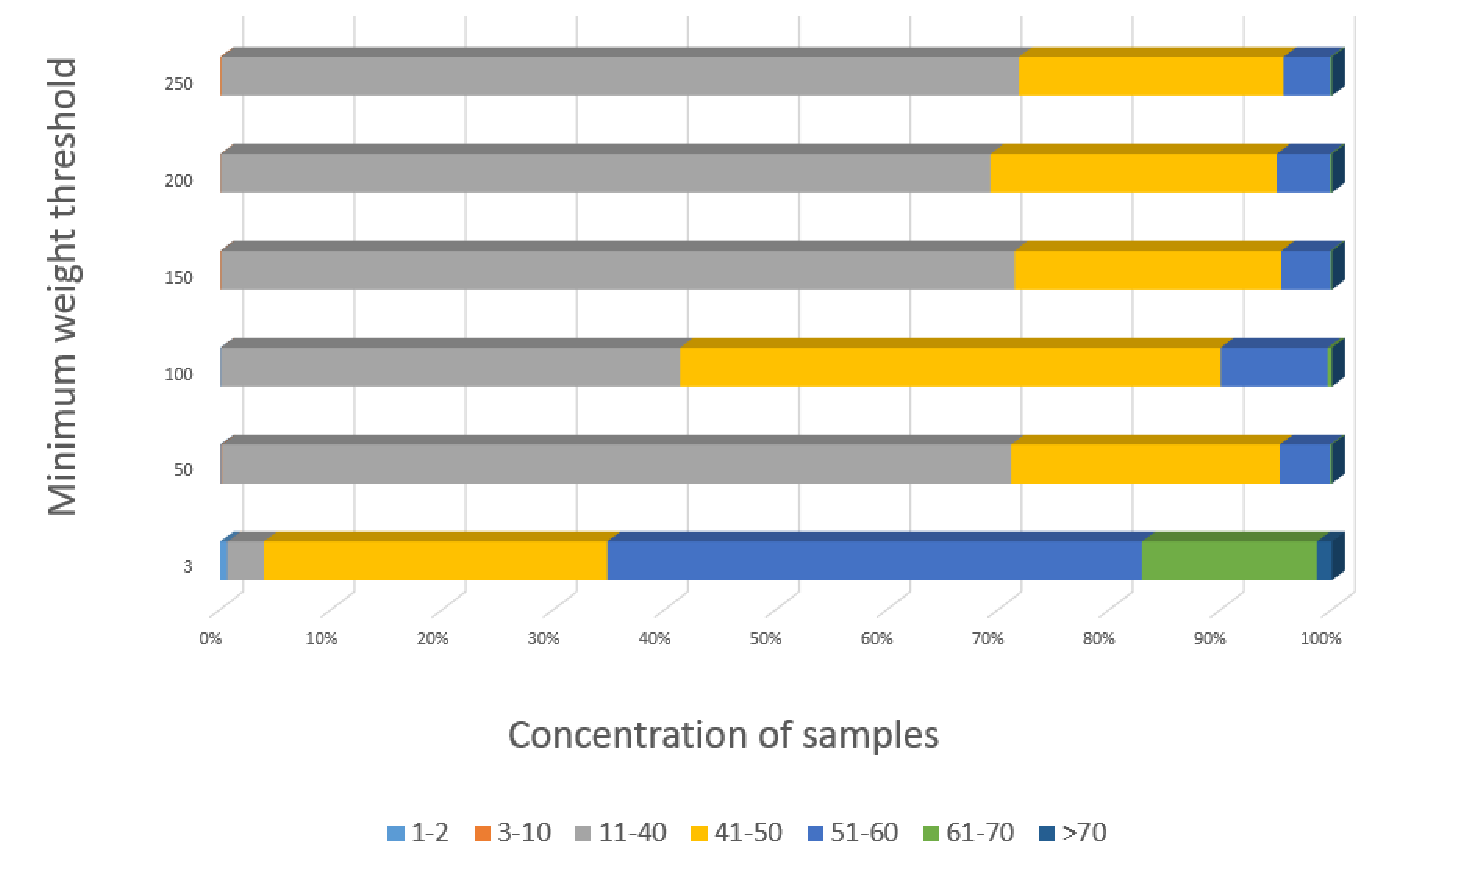
\includegraphics[width=.8\textwidth]{figures/pagetouch-dgenrdm.eps}
		\caption{Frequency of page accesses: Percentage of pages that were accessed a given number of times during a run of the LAMA-CG.}
		\label{fig:pmu-concentsamp-dgenlama}
\end{figure}


Knowing how many times a given page is accessed is very important because in the co-location policy it is necessary to set a threshold of page accesses, for which a page can be judged to belong to a certain home node. Figures \ref{fig:pmu-concentsamp-dgenrdm},\ref{fig:pmu-concentsamp-dgenrdm} and \ref{fig:pmu-concentsamp-dgenrdm} show this information for the distgen-random, distgen-sequential and LAMA-CG respectively. Every bar represents a different value of minimum weight threshold and every color represents the relative percentages of samples that were accessed within the given frequency access interval. It is very important to point out that the number of pages accesses with zero frequency, which are those not accessed by the tool are not depicted. Currently the algorithm has no way of knowing this information and the way to do it is to subtract the total number of pages used by the program memory space from the sum of the total of number pages captured. The number of pages not captured can amount to a significant portion depending on how the sampling is configured.
Every algorithm has its distinctive page access pattern: Distgen sequential has a dominant portion of accesses between 4 and 15 times, distgen-random has a significant portion between 11 and 50 and LAMA-CG has a significant portion of accesses for values as high as 60. Section XYZ presents the results of varying the threshold of page accesses for which a page is identified to belong to a certain node.



\subsection{Completion Time of the Move Pages Call}\label{subsection:pmu-movpatime}


The \textit{move\_pages} directive plays a very important role in the SPM tool because it provides the means to reallocate one page from one node to another, as well as querying in which node a given page, or pages reside in. Figure \ref{fig:mov-pages-time.eps} shows the behavior of such call as function of the number of pages to move. Two scenarios are measured: the first one is the relocation of the pages in conditions of such process running exclusively on the system, and the other is the same relocation together with a distgen process using all the cores, which represents a congestion scenario. It can be seen that for a small number of pages this behavior is almost lineal, but it has an inflection point where the function completion time tends to show a smaller growth with increasing move set size. For the congestion scenario, the function takes longer to complete. In more elaborate scenarios as the ones shown here, the function could take longer to complete, figures in the order of four seconds were measured with scenarios of moving pages in multiple directions with move sizes of 200 thousand samples.

\begin{figure}[th]  
	\centering
		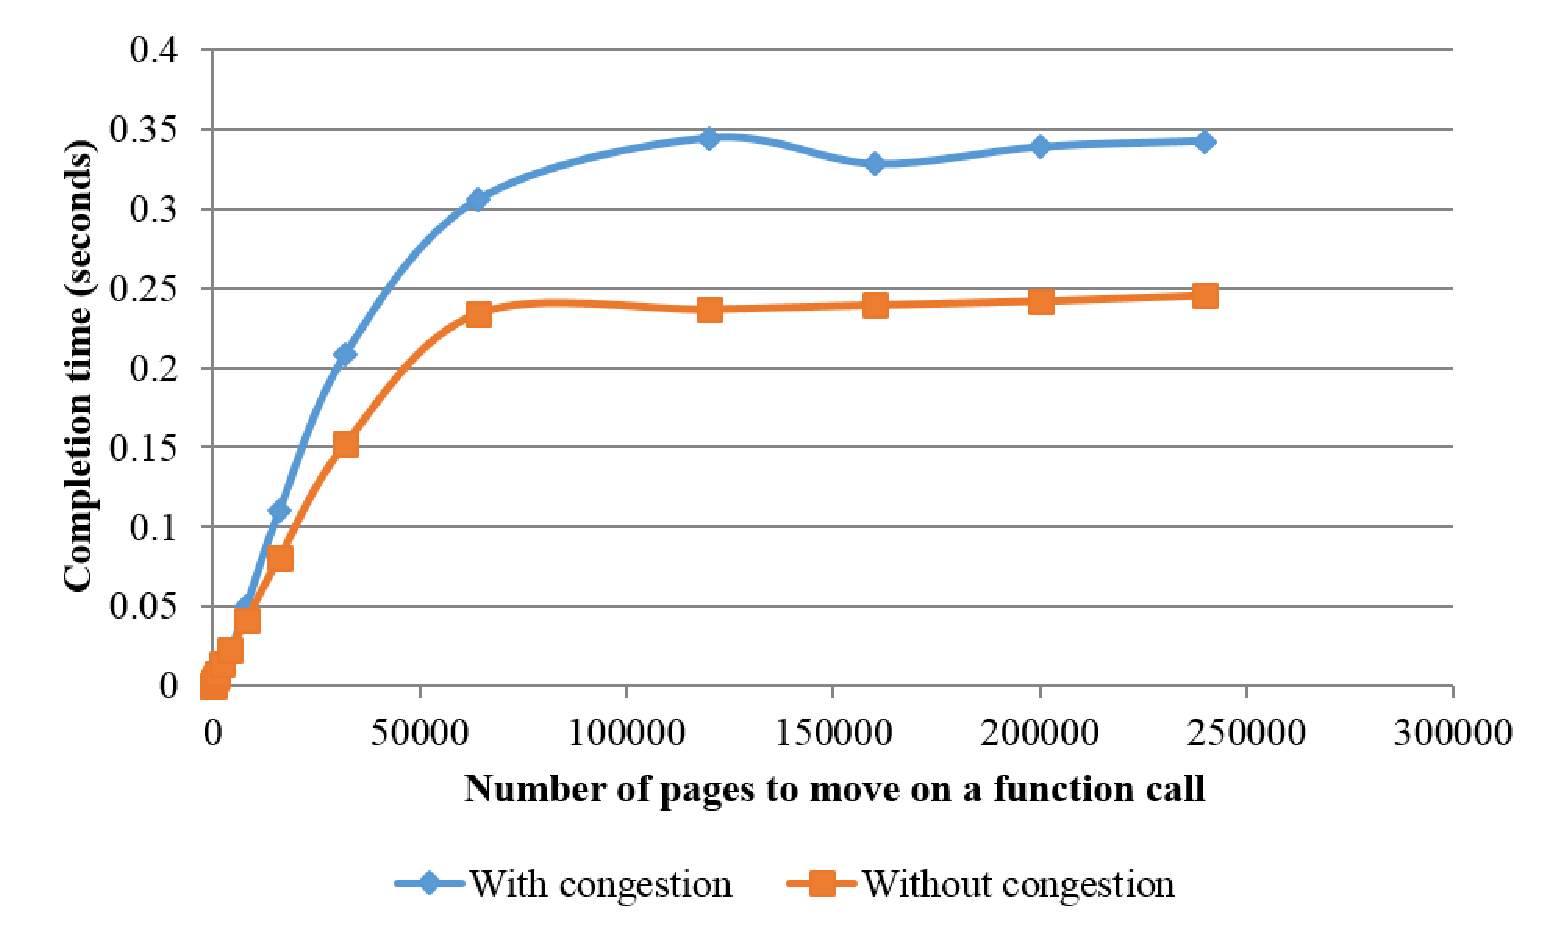
\includegraphics[width=.8\textwidth]{figures/mov-pages-time.eps}
		\caption{Completion times for the move pages call for different page count under contention and no load scenarios for the distgen-random scenario.}
		\label{fig:mov-pages-time.eps}
\end{figure}
